

% \begin{tikzpicture}[remember picture,overlay]    \draw[seahorse] (10.5,0.75) -- (10.5,-6.75); \end{tikzpicture}


\begin{minipage}{0.65\textwidth}

\begin{figure}[ht]
    \centering
    \subfigure[]{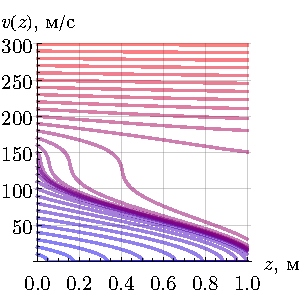
\includegraphics[scale=0.7]{../MOT/figs/vz_v2.pdf}}
    \hspace{5 mm} 
    \subfigure[]{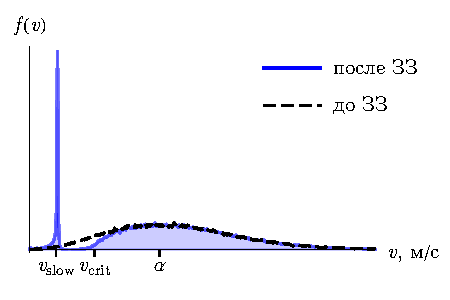
\includegraphics[scale=0.7]{../MOT/figs/vdist_v5.pdf}}
    % zeeman_sim_v2
    \caption{a) Зависимость скорости атомов от координаты в зеемановском замедлителе  для различных начальных скоростей. б) Характерное преобразование распределения атомов по скоростям после замедления. }
\end{figure}


\end{minipage}
\hfill
\begin{minipage}{0.31\textwidth}

Тормозящая сила:
\begin{equation*}
    F = \frac{\hbar k \Gamma}{2} \frac{s}{1+s+4({\delta}+k v)^2/\Gamma^2}
\end{equation*}

\phantom{42}

Уравнение движения:
\begin{equation*}
    \frac{d v}{d t} = \frac{F}{m},
    \hspace{0.1cm} \overset{v \d t = \d z}{\Leftrightarrow}  \hspace{0.1cm}
    \frac{d v}{d z} = \frac{F(v, z)}{m \, v(z)}
\end{equation*}



\end{minipage}